\documentclass[12pt]{article}
\usepackage{amsfonts, amssymb, amsmath, amsthm}
\usepackage[margin=1in]{geometry}
\usepackage{tikz}

\title{Explainer: Problem 6 (Rudin 7.4) --- Analyzing $\sum \frac{1}{1+n^2 x}$}
\author{}
\date{}

\begin{document}
\maketitle

\section*{The series}
$$
f(x) = \sum_{n=1}^{\infty} \frac{1}{1 + n^2 x}.
$$
You need to answer five questions:
\begin{enumerate}
  \item For what $x$ does the series converge absolutely?
  \item Where does it converge uniformly?
  \item Where does it fail to converge uniformly?
  \item Is $f$ continuous where the series converges?
  \item Is $f$ bounded?
\end{enumerate}

\section*{First: where can it even converge?}
Look at the $n$th term: $\frac{1}{1 + n^2 x}$.
\begin{itemize}
  \item \textbf{$x > 0$:} Term behaves like $1/(n^2 x)$, so compare with $\sum 1/n^2$. \textbf{Converges absolutely.}
  \item \textbf{$x = 0$:} Each term is $1$. $\sum 1$ diverges.
  \item \textbf{$x < 0$:} Then $1 + n^2 x = 0$ exactly when $n^2 = -1/x$. So if $-1/x$ is a perfect square, a term is undefined. Otherwise the terms grow like $-1/(n^2 |x|)$ and the sum converges. But you must \emph{exclude} the reciprocals of negative squares: $x \neq -1/n^2$ for any $n$.
\end{itemize}

\begin{center}
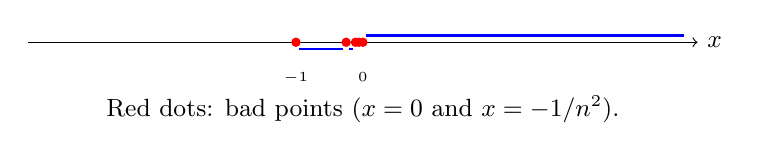
\begin{tikzpicture}[scale=0.85]
  \draw[->] (-5, 0) -- (5, 0) node[right] {\small $x$};
  \foreach \n in {1,2,3,4} {
    \pgfmathsetmacro\val{-1/(\n*\n)}
    \fill[red] (\val, 0) circle (2pt);
  }
  \fill[red] (0, 0) circle (2pt);
  \draw[thick, blue] (0.05, 0.1) -- (4.8, 0.1);
  \draw[thick, blue] (-0.95, -0.1) -- (-0.30, -0.1);
  \draw[thick, blue] (-0.20, -0.1) -- (-0.15, -0.1);
  \node[below] at (0, -0.3) {\tiny $0$};
  \node[below] at (-1, -0.3) {\tiny $-1$};
  \node at (0, -1) {\small Red dots: bad points ($x=0$ and $x=-1/n^2$).};
\end{tikzpicture}
\end{center}

\section*{Uniform convergence}
Use the \textbf{Weierstrass $M$-test}: if $|\text{term}_n(x)| \leq M_n$ with $\sum M_n < \infty$, then uniform convergence.

\textbf{On $[\delta, \infty)$ for any $\delta > 0$:} bound $\left|\frac{1}{1+n^2 x}\right| \leq \frac{1}{n^2 \delta}$, $M$-test wins. \textbf{Uniform.}

\textbf{On $(0, \infty)$ (not bounded away from $0$):} as $x \to 0^+$, each term $\to 1$, and any tail $\sum_{n=N}^\infty$ can be forced large by choosing $x$ small. \textbf{Not uniform.}

\textbf{Near negative roots $-1/n^2$:} the individual term $1/(1+n^2 x)$ blows up, so no uniform convergence on any interval containing such a point.

\textbf{On any interval bounded away from $0$ and from every $-1/n^2$:} similar $M$-test argument works.

\section*{Continuity}
Uniform limit of continuous functions is continuous (Theorem 7.12). The series converges uniformly on every compact set avoiding the bad points --- continuity is a \emph{local} property, so $f$ is continuous on its domain.

\section*{Boundedness}
Check behavior as $x \to 0^+$: each term $\to 1$. Partial sums $\to N$ at $x = 0^+$. In fact $f(x) \to +\infty$ as $x \to 0^+$. \textbf{So $f$ is not bounded.}

\section*{Strategy summary}
\begin{enumerate}
  \item Pin down the domain (exclude $x = 0, -1/n^2$).
  \item Use $M$-test on intervals bounded away from the bad points.
  \item Show non-uniformity by exhibiting $x$-values where tails stay $\geq$ some fixed constant.
  \item Continuity from uniform convergence on compact pieces of the domain.
  \item Boundedness: analyze $x \to 0^+$.
\end{enumerate}

\end{document}
